%!TEX root = ../../main.tex
\section{Systemarkitektur}
Under systemarkitektur beskrives den overordnede systemarkitektur som er dokumenteret i projektdokumentationen. Systemarkitekturen fungerer som udviklingsramme for videre design og implementering. Det er her at systemets funktionalitet, der er beskrevet i systembeskrivelsen og kravspecifikationen, nedbrydes til overordnede moduler.
\\\\
Systemet kan illustreres i et BDD bestående af flere moduler. 
\begin{figure}[H]
	\centering
	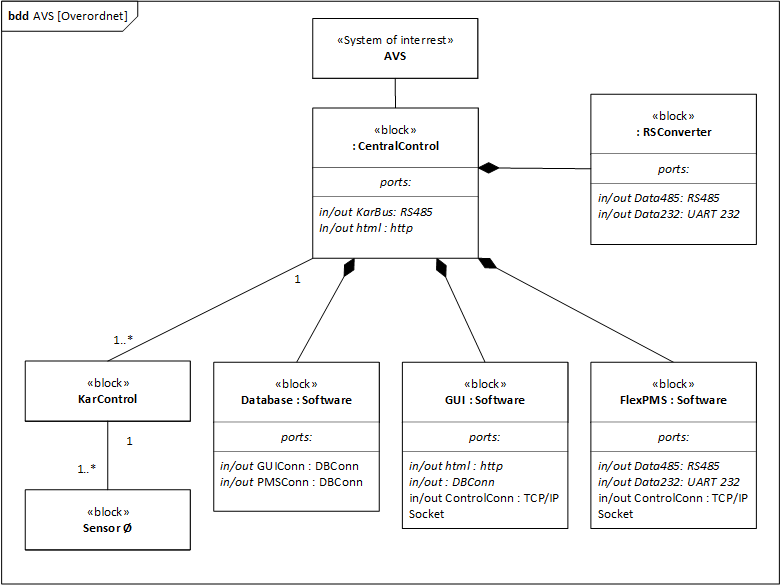
\includegraphics[width=1\textwidth]{Projektbeskrivelse/Systemarkitektur/photo/System_BDD}
	\caption{Block Definition Diagram af AVS}
	\label{fig:System_BDD}
\end{figure} 

\subsection{Blokbeskrivelser af AVS}
Systemmet består af en \textbf{\textit{CentralControl}}, ud fra den er der en \textbf{\textit{RSConverteren}} som konverterer mellem RS485 og UART 232, der er blevet anvendt fordi den giver mulighed for at have en længere afstand mellem systemmet.
\\\\
Gennem \textbf{\textit{GUI}} kan brugeren tilgå systemet.
\\\\
\textbf{\textit{Databasen}} skal indeholde alle sensor data samt de indtastede værdier fra brugeren. 
\\\\
Softwaren som er bindeleddet mellem \textbf{\textit{GUI}} og de andre delsystemer kaldes \textbf{\textit{FlexPMS}}. \textbf{\textit{FlexPMS}} afvikles konstant på \textbf{\textit{CentralControl}}, og håndterer at sende kommandoer til og opsamle data fra \textbf{\textit{KarControl}}.
\\\\
Der kan være en til flere \textbf{\textit{KarControler}}, som har til arbejde at styr og håndterer al datakommunikation og kommandoer relateret til ét kar.
\\\\
Ud fra \textbf{\textit{KarControl}} kan der være en til flere \textbf{\textit{Sensor Øer}} der giver mulighed for at måle (f.eks. jordfugtighed) over et større areal ved, at \textbf{\textit{Sensor
Ø’erne}} spredes over området, hvor planterne gror, og har hver især tilsluttet sensorer.

\subsection{Allokerings diagram af AVS}
I AVS er der en række blokke der har en logisk funktionalitet, som er allokeret på en række fysiske enheder. Nedenstående diagram viser hvor de logiske blokke er allokeret.

\begin{figure}[H]
	\centering
	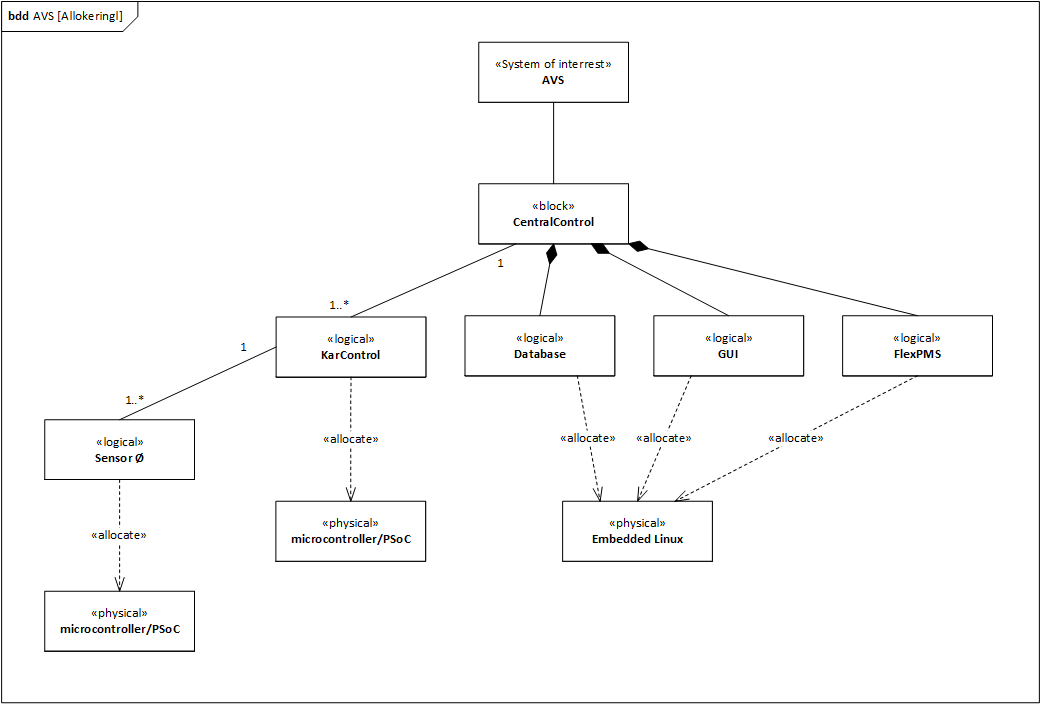
\includegraphics[width=1\textwidth]{Projektbeskrivelse/Systemarkitektur/photo/System_Allokeringsdiagram}
	\caption{Allokerings diagram af AVS}
	\label{fig:System_BDD}
\end{figure} 
Det ses på diagrammet at KarControl og SensorØ er allokeret på hver deres microkontroller/PSoC. I dette projekt er det besluttet at microcontrolleren skal
være af typen PSoC4.  \\
Databasen , GUI og Flex er allokeret på Embedded Linux. 
